%
%  module_IV.tex
%
%  Created by Drew Conway on 2010-06-01.
% 
%
\documentclass[xcolor=dvipsnames, 9pt]{beamer}

\newenvironment{code}{\begin{semiverbatim} \begin{footnotesize}}
{\end{footnotesize}\end{semiverbatim}}

\usepackage{graphicx}
\usepackage{amssymb}
\usepackage{amsfonts}
\usepackage{amsmath}
\usepackage{hyperref}
\usepackage{natbib}
\usepackage{color}
\usepackage{pdfsync}
\usepackage{chancery}
\usepackage{movie15}
\usepackage{pgfpages}
\usepackage{fancyvrb}
\usepackage{colortbl}

% \definecolor{white}{rgb}{255,255,255}
% \definecolor{darkred}{rgb}{0.5,0,0}
% \definecolor{darkgreen}{rgb}{0,0.5,0}
% \definecolor{lightblue}{rgb}{0,0,0.7}

% \hypersetup{colorlinks,
%   linkcolor=white,
%   filecolor=darkred,
%   urlcolor=lightblue,
%   citecolor=darkblue}

\usepackage{beamerthemesplit}
\usetheme{Copenhagen}
\usecolortheme[named=Violet]{structure} 
\setbeamertemplate{navigation symbols}{}
\setbeamertemplate{itemize items}[triangle]
\setbeamertemplate{enumerate items}[default]
%\setbeameroption{show notes on second screen}
%\logo{\includegraphics[width = 2cm]{nyulogo.png}}

\newcommand{\R}{\mathbb{R}}
\renewcommand{\d}{\mathsf{d}}
\newcommand{\dd}{\partial}
\newcommand{\E}{\mathsf{E}}
\newcommand{\bb}{\mathbf}

\title{Module IV - Basic Analysis}
\author{Drew Conway --- Department of Politics}
\institute{
\includegraphics[width = 4cm]{../images/logos/500px-NYU_logo.png}}
\date{June 29, 2010}

\begin{document} 

\begin{frame}[plain]
  \titlepage  
\end{frame}

\begin{frame}
	\frametitle{Agenda for Module IV}
	Loading data from multiple sources
	\begin{itemize}
	   \item Local network data files
	   \item Connecting to a database
	   \item Building directly from the Internet
	\end{itemize}
	\uncover<2->{Brief review of Python dictionaries
	\begin{itemize}
	   \item Why is the \texttt{dict} so useful?
	   \item How \texttt{NetworkX} utilizes it?
	\end{itemize}}
	\uncover<3->{Running basic centralities
	\begin{itemize}
	   \item Degree, Closeness, Betweeness Eigenvector
	   \item Calculating degree distribution
	   \item Plotting statistics using \texttt{matplotlib}
	   \item Calculating cliques, clustering and transitivity
	\end{itemize}}
	\uncover<4->{Outputting data into multiple formats
	\begin{itemize}
	   \item Writing network data
	   \item Saving network analysis statistics
	\end{itemize}}
	\uncover<5->{Basic visualization
	\begin{itemize}
	   \item Review of \texttt{NetworkX}'s plotting algorithms
	   \item Adding analysis to visualization 
	\end{itemize}}
\end{frame}

\section{Loading data from multiple sources} % (fold)
\label{sec:loading_data_from_multiple_sources}

\subsection{Local network data} % (fold)
\label{sub:local_network_data}

\begin{frame}[fragile]
    \frametitle{Loading a network file}
    As we have seen, one of the main advantages of working with \texttt{NetworkX} is that it can read many different network formats
    \begin{itemize}
        \item For those that are unfamiliar with working at the \textbf{command-line}, however, the process can be confusing
    \end{itemize}
    \begin{block}{NX syntax for loading a file}
        \begin{tabular}{cccc}
        \alert<2>{$>>> G$} & = & \alert<3>{read\_format(``path/to/file.txt''}, & \alert<4>{\emph{...options...}}) \\
        \alert<2>{\uparrow} & & \alert<3>{\uparrow} & \alert<4>{\uparrow} \\
        \alert<2>{\scriptsize{Net variable}} & & \alert<3>{\scriptsize{NX function, file directory path}} & \alert<4>{\scriptsize{Graph type, nodes type, etc.}}
        \end{tabular}
    \end{block}
    \uncover<5->{Let's try!
    \begin{itemize}
        \item We will load the edge list of Hartford drug users network
        \item Specify that the network be a directed graph, and the nodes be integers
        \item Use \texttt{info()} to check that data has been loaded correctly
    \end{itemize}}
    \begin{center}
        \uncover<6->{\alert<6>{It's time to fire up your console and load Python!}}
    \end{center}
\end{frame}

\begin{frame}[fragile]
    \frametitle{Loading the Hartford drug users network}
    \begin{block}{Starting \texttt{NetworkX} and loading data}
        \begin{code}
\scriptsize{>>> from networkx import *
>>> hartford=\alert<3>{read_edgelist}("\alert<4>{../../data/hartford_drug.txt}",\alert<5>{create_using=DiGraph()},\alert<6>{nodetype=int})
>>> \alert<7>{info(hartford)}
Name:                  
Type:                  DiGraph
Number of nodes:       212
Number of edges:       337
Average in degree:     1.5896
Average out degree:    1.5896}
        \end{code}
    \end{block}
\uncover<2->{What did we just do?}
\begin{itemize}
    \item \uncover<3->{Used the \texttt{read\_edgelist} function to load EL file}
    \item \uncover<4->{Specified path to Hartford drug users file}
    \item \uncover<5->{Used the \texttt{create\_using} option to force NX to create as a directed graph}
    \item \uncover<6->{Used the \texttt{nodetype} option to force NX to store nodes as integers}
    \item \uncover<7->{Used the \texttt{info} function to check that it all worked}
\end{itemize}
\uncover<8->{Some formats may have more or less options, \textbf{always check the documentations!}}
\end{frame}

% subsection local_network_data (end)

\subsection{Connecting to a database} % (fold)
\label{sub:connecting_to_a_database}

\begin{frame}[fragile]
    \frametitle{Building a network from a database}
    As data sets become larger and persistently changing, it may make more sense to store them in a database rather than a single file
    \begin{itemize}
        \item As we have seen, Python provides binding to many modern database frameworks
    \end{itemize}
\end{frame}


% subsection connecting_to_a_database (end)

\subsection{Building directly from the Internet} % (fold)
\label{sub:building_directly_from_the_internet}

\begin{frame}[fragile]
    \frametitle{Building the social network among LiveJournal users}
    \begin{columns}
        \column{.5\textwidth}
            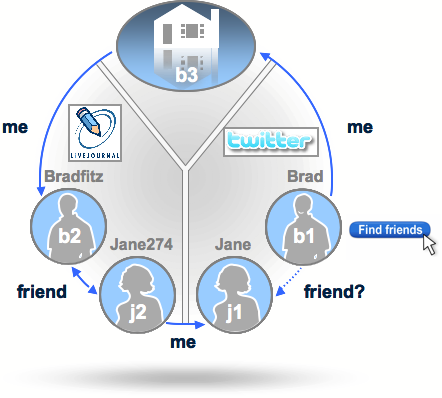
\includegraphics[scale=0.38]{../images/logos/find-a-friend.png}
        \column{.5\textwidth}
       Perhaps the most powerful aspect of NetworkX is its ability to work in Python to generate networks from live-streaming data
        \begin{itemize}
            \uncover<2->{\item In Python, use \texttt{NetworkX}, \texttt{cjson} and a other standard scientific libraries to parse Google's SocialGraph data }
            \uncover<3->{\item Using a ``seed'' user, we will build out a network}
            \uncover<4->{\item Through a process called ``k-snowball searching'' $seed\rightarrow friend\rightarrow\dots\rightarrow friend_{k}$}
            \uncover<5->{\begin{itemize}
                \scriptsize{\item Seed: \href{http://imichaeldotorg.livejournal.com/}{imichaeldotorg.livejournal.com}
                \item $k = 3$}
            \end{itemize}}
            \uncover<6->{\item \alert{Note the low value of $k$}}
        \end{itemize}
    \end{columns}
\end{frame}

\begin{frame}[fragile]
    \frametitle{The code, part 1}
    \begin{columns}
        \column{.5\textwidth}
        \begin{block}{\scriptsize{Loading the libraries and setting things up}}
            \begin{code}
\tiny{from cjson import *
from urllib import *
from networkx import *
from time import *
from scipy import array,unique
...
if __name__ == "__main__":
    seed_url=``http://imichaeldotorg.livejournal.com"
    sg=get_sg(seed_url)
    net,newnodes=create_egonet(sg)
    info(net)}
                \end{code}
            \end{block}}
        \column{.5\textwidth}
\begin{code}
\uncover<2->{\tiny{Name:                  [`http://imichaeldotorg.livejournal.com/']
Type:                  DiGraph
Number of nodes:       5
Number of edges:       5
Average in degree:     1.0
Average out degree:    1.0}}
\end{code}
    \end{columns}
    \begin{block}{\scriptsize{Get the JSON from SocialGraph}}
        \begin{code}
    \tiny{def get_sg(seed_url):
        sgapi_url="http://socialgraph.apis.google.com/lookup?q="+seed_url+"&edo=1&edi=1&fme=1&pretty=0"
        try:
            furl=urlopen(sgapi_url)
            fr=furl.read()
            furl.close()
            return fr
        except IOError:
            print "Could not connect to website"
            print sgapi_url
            return {}}
        \end{code}
    \end{block}    
\end{frame}

\begin{frame}[fragile]
    \frametitle{Build egonet and snowball}
    \begin{columns}
        \column{0.4\textwidth}
        \begin{block}{\scriptsize{Creating the egonet}}
            \begin{code}
\tiny{def create_egonet(s):
    try:
        raw=decode(s)
        G=DiGraph()
        pendants=[]
        n=raw['nodes']
        nk=n.keys()
        G.name=str(nk)
        pendants=[]
        for a in range(0,len(nk)):
            for b in range(0,len(nk)):
                if a!=b:
                    G.add_edge(nk[a],nk[b])
        for k in nk:
            ego=n[k]
            ego_out=ego['nodes_referenced']
            for o in ego_out:
                G.add_edge(k,o)
                pendants.append(o)
            ego_in=ego['nodes_referenced_by']
            for i in ego_in:
                G.add_edge(i,k)
                pendants.append(i)
        pendants=array(pendants,dtype=str)
        pendants.flatten()
        pendants=unique(pendants)
        return G,pendants
    except DecodeError:
    ...
    except KeyError:}
            \end{code}
        \end{block}
        \column{0.6\textwidth}
        \begin{block}{\scriptsize{Rolling the snowball}}
            \begin{code}
\tiny{def snowball_round(G,seeds,myspace=False):
    t0=time()
    if myspace:
        seeds=get_myspace_url(seeds)
    sb_data=[]
    for s in range(0,len(seeds)):
        s_sg=get_sg(seeds[s])
        new_ego,pen=create_egonet(s_sg)
        for p in pen:
                sb_data.append(p)
        if s<1:
            sb_net=compose(G,new_ego)
        else:
            sb_net=compose(new_ego,sb_net)
        del new_ego
        if s==round(len(seeds)*0.2):
            sb_net.name='20% complete'
            sb_net.info()
            print 'AT: '+strftime('%m/%d/%Y, %H:%M:%S', gmtime())
            print ''
    ...
    # More time keeping, probably a MUCH better way to do this
    sb_data=array(sb_data)
    sb_data.flatten()
    sb_data=unique(sb_data)
    sb_net.info()
    return sb_net,sb_data}
            \end{code}
        \end{block}
    \vspace{5mm}
    \end{columns}
\end{frame}

\begin{frame}[fragile]
    \frametitle{Build the whole network}
    \begin{columns}
        \column{0.5\textwidth}
         \scriptsize{\begin{tabular}{l|l|l|l|l}
         Step & Nodes & Edges & Mean Degree & Density \\ \hline \hline
         \color<2>{red}{Seed} & \color<2>{red}{5} & \color<2>{red}{5} & \color<2>{red}{2.0} & \color<2>{red}{0.25} \\ \hline
         \color<3>{red}{$k=2$} & \color<3>{red}{75} & \color<3>{red}{115} & \color<3>{red}{3.0} & \color<3>{red}{0.02} \\ \hline
         \color<4>{red}{$k=3$} & \color<4>{red}{4,938} & \color<4>{red}{8,659} & \color<4>{red}{3.5} & \color<4>{red}{$3.6(10^{-4})$}
         \end{tabular}}
         \column{0.5\textwidth}
         \begin{itemize}
            \item \uncover<2->{\scriptsize{Our seed is abnormally isolated, with only four neighbors}}
            \item \uncover<3->{\scriptsize{Large jump after first snowball}}
            \item \uncover<4->{\scriptsize{Massive structural leap at $k=3$}}
         \end{itemize}
    \end{columns}
    \begin{center}
        \uncover<3->{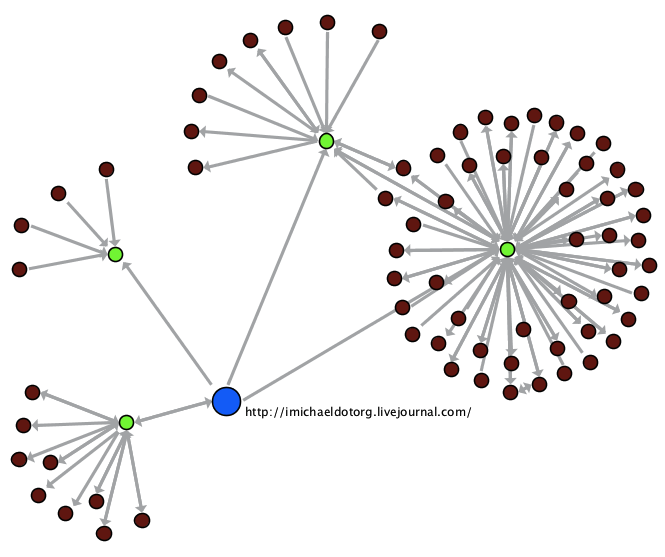
\includegraphics[scale=0.3]{../images/networks/goog_api_k2.png}}
    \end{center}
\end{frame}

\begin{frame}[fragile]
    \frametitle{The full network}
    To get a feeling for the size of the full network...
    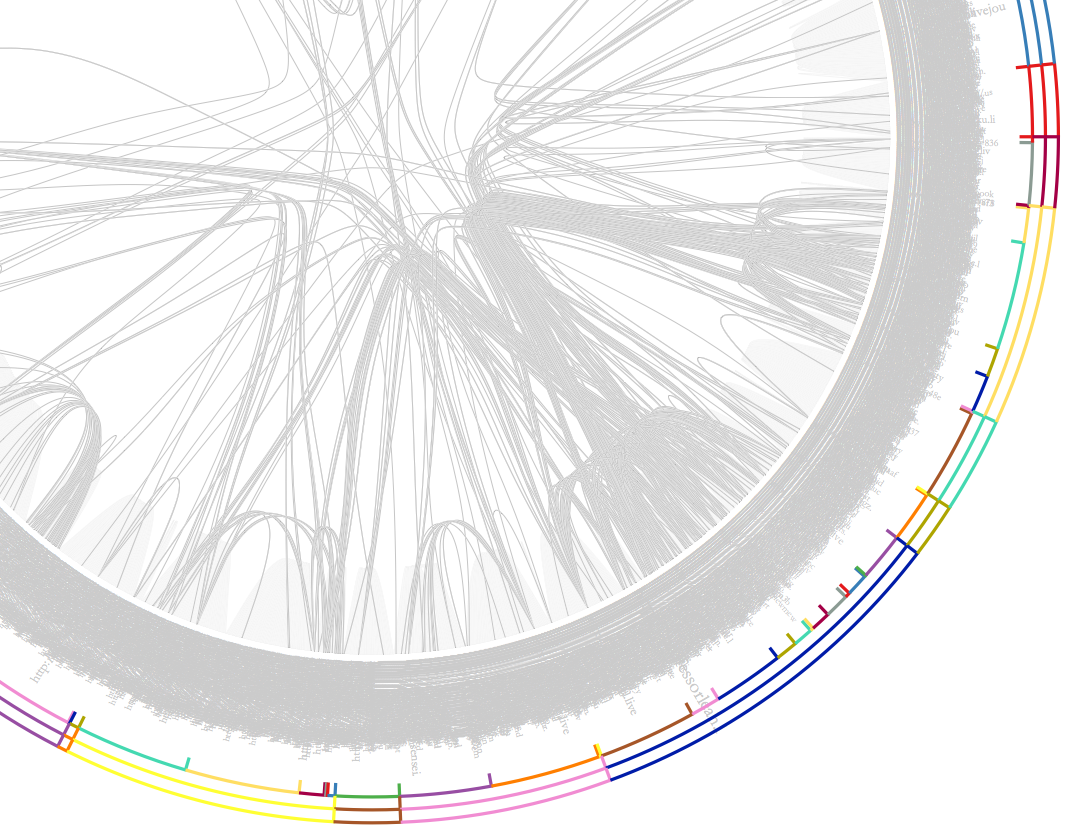
\includegraphics[scale=0.3]{../images/networks/big_wheel.png}
\end{frame}

% subsection building_directly_from_the_internet (end)

% section loading_data_from_multiple_sources (end)

\section{The Python \texttt{dict}} % (fold)
\label{sec:the_python_dict}

\subsection{Overview of the \texttt{dict} data type} % (fold)
\label{sub:overview_of_the_dict}

\begin{frame}[fragile]
    \frametitle{Python Dictionaries}
    \uncover<1->{The \texttt{dict} type is a data structure that represents a key$\rightarrow$value mapping}
    \uncover<2->{\begin{block}{Working with the dict type}}
        \begin{code}
\uncover<2->{\alert<2>{\# Keys and values can be of any data type}}
\uncover<2->{>>> fruit\_dict=\{"apple":1,"orange":[0.23,0.11],"banana":True \}} \newline
\uncover<3->{\alert<3>{\# Can retrieve the keys and values as Python lists (vector)}
>>> fruit\_dict.keys()
["orange","apple","banana"]} \newline
\uncover<4->{\alert<4>{\# Or create a (key,value) tuple}
>>> fruit\_dict.items()
[("orange",[0.23,0.11]),("apple",1),("Banana",True)]}
\uncover<5->{\alert<5>{\# This becomes especially useful when you master Python ``list comprehension''}}
            \end{code}
        \end{block}
\uncover<6->{The Python dictionary is an extremely flexible and useful data structure, making it one of the primary advantages of Python over other languages
\begin{itemize}
    \item This is particularly useful when performing analysis on networks, where node labels are natural keys
\end{itemize}}
\uncover<7->{\begin{center}
    \alert{Now, try creating a \texttt{dict} of your own}
\end{center}}
\end{frame}

% subsection overview_of_the_dict (end)

\subsection{How NetowrkX uses the \texttt{dict}} % (fold)
\label{sub:how_netowrkx_uses_the_dict}

\begin{frame}[fragile]
    \frametitle{Using dictionaries for network analysis}
    \begin{columns}
        \column{.45\textwidth}
        From the documentation...\\ \vspace{3mm}
        \only<1>{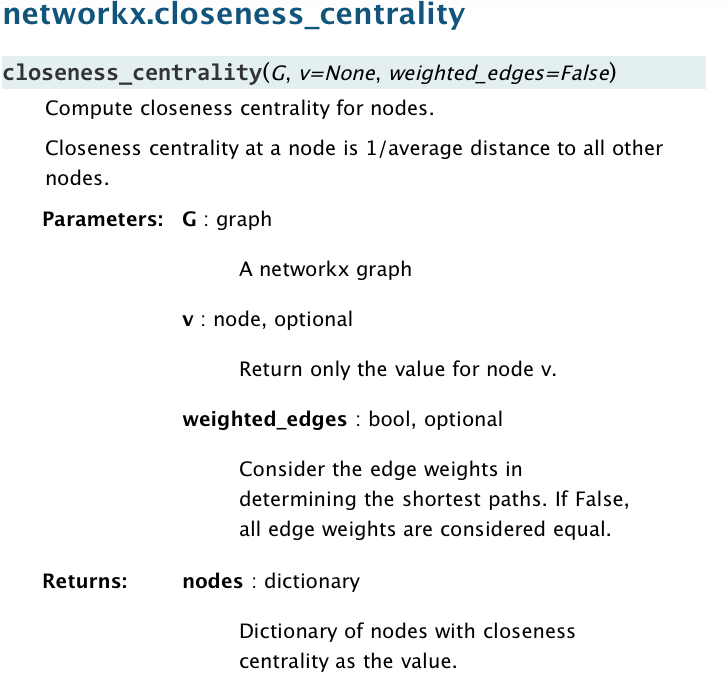
\includegraphics[width=5cm]{../images/figures/closeness_doc.png}}\only<2>{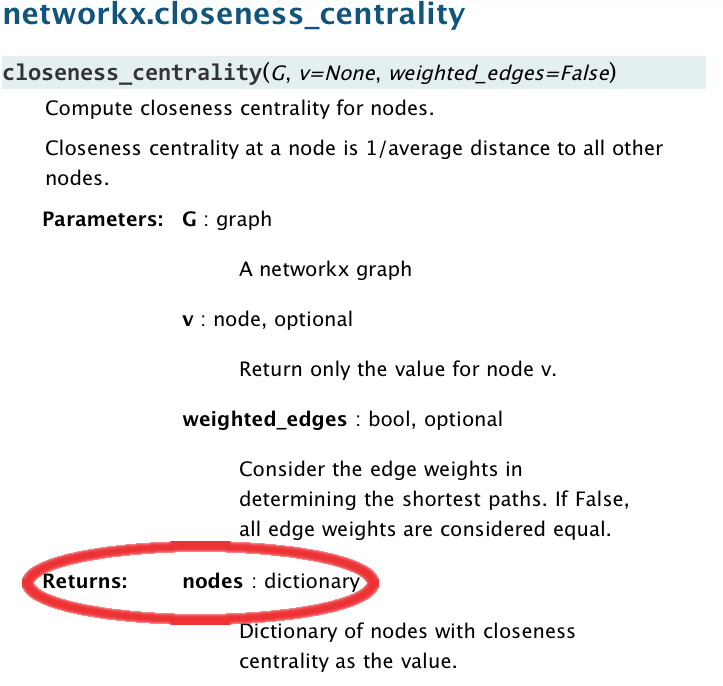
\includegraphics[width=5cm]{../images/figures/closeness_doc_2.png}}
        \column{.55\textwidth}
        \texttt{NetworkX}'s metric's make extensive use of the dict type
        \begin{itemize}
            \item In this case the key$\rightarrow$value mapping is of the form: \texttt{\{node\_label: metric\}} 
        \end{itemize}
        Let's look at an example:
        \begin{block}{In-degree centrality of Hartford data}
            \begin{code}
\scriptsize{>>> in_cen=in_degree_centrality(hartford)
>>> in_cen
\{1: 0.014218009478672987, 2: 0.018957345971563982,...
...
90: 0.0047393364928909956, 293: 0.0\}}
            \end{code}
        \end{block}
        We can see that node \#90 has in-degree centrality 0.0047
        \begin{itemize}
            \item But we can do so much more!
        \end{itemize}
    \end{columns}
\end{frame}

% subsection how_netowrkx_uses_the_dict (end)

% section the_python_dict (end)

\section{Running basic centralities} % (fold)
\label{sec:running_basic_centralities}

\subsection{Calculating centralities} % (fold)
\label{sub:calculating_centralities}

\begin{frame}[fragile]
    \frametitle{Running multiple measures}
    For our first analysis in NetworkX, we will do some basic network manipulation, then run multiple measures to find highest centrality nodes
    \begin{itemize}
        \item First, we will need to convert to an undirected network, and extract the main component
    \end{itemize}
    \begin{block}{Find main component \& symmetrize}
        \begin{code}
# Many of the centrality metrics require undirected graphs, so we will symmetrize
>>> \alert<2>{hartford_ud=hartford.to_undirected()}
# The network also has many small components, but for
# this analysis we are interested in the largest
>>> \alert<3>{hartford_mc=hartford_main=connected_component_subgraphs(hartford_ud)[0]}
        \end{code}
    \end{block}
    Next, we will calculate multiple measures
    \begin{block}{Computing multiple centralities}
        \begin{code}
# Betweenness centrality
>>> \alert<4>{bet_cen=betweenness_centrality(hartford_mc)}
# Closeness centrality
>>> \alert<4>{clo_cen=closeness_centrality(hartford_mc)}
# Eigenvector centrality
>>> \alert<4>{eig_cen=eigenvector_centrality(hartford_mc)}
        \end{code}
    \end{block}
\end{frame}

\begin{frame}[fragile]
    \frametitle{Finding most central actors}
    To find the most central actors we will use Python's list comprehension technique to do basic data manipulation on our centrality dictionaries
    \begin{columns}
        \column{.6\textwidth}
            \begin{block}{Function for finding most central actor}
        \begin{code}
def highest_centrality(cent_dict):
    """Returns node key with largest value from
    NX centrality dict"""
    \alert<2>{# Create ordered tuple of centrality data
    cent_items=cent_dict.items()}
    \alert<3>{# List comprehension!
    cent_items=[(b,a) for (a,b) in cent_items]}
    \alert<4>{# Sort in descending order
    cent_items.sort()
    cent_items.reverse()
    return cent_items[0][1]}
        \end{code}
            \end{block}
            \column{.4\textwidth}
            \uncover<3->{List comprehension
            \begin{itemize}
                \scriptsize{\item Given a dict: \texttt{d=\{1: 0.15, 2: 0.67\}}}
                \scriptsize{\item \texttt{d.items()} $\rightarrow$ \texttt{[(1,0.15),(2,0.67)]}}
                \scriptsize{\item \texttt{d=[(b,a) for (a,b in d)]} $\rightarrow$ \texttt{[(0.15,1),(0.67,2)]}}
            \end{itemize}}}
            \uncover<4->{Here, we use list comprehension in order to use Python's built-in \texttt{sort} and \texttt{reverse} list functions}
    \end{columns}
    \vspace{2mm}Now, just ask for the answer
    \begin{block}{Finding Most central actors}
        \begin{code}
\scriptsize{>>>  print("Actor "+str(highest_centrality(bet_cen))+" has the highest Betweenness centrality")
\alert<5->{Actor 82 has the highest Betweenness centrality}}
        \end{code}
    \end{block}
\end{frame}


% subsection calculating_centralities (end)

% section running_basic_centralities (end)

\end{document}
